\Problem[1]{Maximum Tilt}{\MaximumTilt}{
A block is placed on an inclined plane and the angle of the plane is adjusted until the block just begins to slide. The coefficient of static friction is 0.35 and the coefficient of kinetic friction is 0.25.
}
\ProblemSub{\MaximumTiltA}{
(a) Draw a sketch illustrating the problem.
}
\Solution{\MaximumTiltASol}{
\begin{figure}[h]
	\centering
	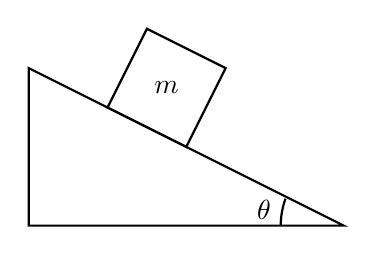
\begin{tikzpicture}
		\draw[thick] (0,0) -- (4,0) -- (0,2) -- cycle;
		\draw[thick] (3.2,0) arc (180:160:1);
		\node[anchor=east] at (3.2,0.2) {$\theta$};
		\draw[thick] (1,1.5) -- (2,1) -- (2.5,2) -- (1.5,2.5) -- cycle;
		\node at (1.75,1.75) {$m$};
	\end{tikzpicture}
\end{figure}
}
\ProblemSub{\MaximumTiltB}{
(b) Draw a free-body diagram for the block. Use the particle model with tilted axes.
}
\Solution{\MaximumTiltBSol}{
\begin{figure}[h]
	\centering
	\begin{tikzpicture}
		\FBDaxes{0,0}{-20}{axes}
		\draw[thick,dashed] (1.8,-0.68) -- (0.4,-0.68);
		\draw[thick] (1,-0.68) arc (180:160:0.8);
		\node[anchor=east] at (1,-0.48) {$\theta$};
		\FBDvectorMA{axes}{1.41}{70}{FN}
		\node[anchor=west] at (FNtip) {$\vec{F}^{N}_{BR}$};
		\FBDvectorMA{axes}{0.42}{160}{FF}% 0.49 for static, 0.35 for kinetic
		\node[anchor=south] at (FFtip) {$\vec{F}^{f}_{BR}$};
		\FBDvectorXY{axes}{0,-1.5}{FG}
		\draw[thick] (0,-0.8) arc (270:250:0.8);
		\node[anchor=north] at (-0.2,-0.8) {$\theta$};
		\node[anchor=west] at (FGtip) {$\vec{F}^{g}_{BE}$};
		\FBDdot{axes}
	\end{tikzpicture}
\end{figure}

The diagram is qualitatively accurate for both the static and kinetic friction cases, though the friction vector may vary in size depending on which case we are looking at. Since there are no forces of the same type, I will drop the subscripts for the remainder of the problem (i.e. $F^{g}_{BE}$ will just be $F^{g}$, and so on).
}
\ProblemSub{\MaximumTiltC}{
(c) Find the angle at which the block just begins to slide.
}
\Solution{\MaximumTiltCSol}{
At the maximum angle for which the block doesn't slide, the force of static friction attains its maximum value. Tilting the surface even infinitesimally further, or giving the block the lightest push, will cause it to begin sliding. For now, both the $ x $ and $ y $ components of acceleration are zero. From the $ y $-components, we recover the normal force:
\[
\begin{split}
	F^{net}_{y} & = ma_{y} \\
	F^{N} + F^{g}_{y} & = 0 \\
	(F^{g}_{y} & = -mg\cos\theta) \\
	F^{N} & = -F^{g}_{y} = mg\cos\theta.
\end{split}
\]
This tells us that $ F^{sf}_{max} = \mu_{s}F^{N} = \mu_{s}mg\cos\theta $. We use this in the $ x $-component calculations:
\[
\begin{split}
	F^{net}_{x} & = ma_{x} \\
	F^{g}_{x} - F^{sf}_{max} & = 0 \\
	F^{sf}_{max} & = F^{g}_{x} = mg\sin\theta \\
	\mu_{s}\cancel{mg}\cos\theta & = \cancel{mg}\sin\theta \\
	\mu_{s} & = \frac{\sin\theta}{\cos\theta} = \tan\theta
\end{split}
\]
Now we can solve for the maximum angle:
\[
\theta = \arctan(\mu_{s}) = \arctan(0.35) \approx 19^{\circ} \text{ (2 sig figs)}.
\]
The maximum angle (accounting for significant figures) is 19$ ^{\circ} $, though we should carry the less approximate angle 19.3$ ^{\circ} $ through any further calculations.
}
\ProblemSub{\MaximumTiltD}{
(d) Keeping the angle the same, find the acceleration of the block after it starts to slide.
}
\Solution{\MaximumTiltDSol}{
Now, the friction is kinetic, and therefore it is smaller than the maximum static friction. This results in a net force and acceleration down the plane. The $ y $-component of acceleration is still zero, so we still have $ F^{N} = mg\cos\theta $. In the $ x $ direction, we have
\[
\begin{split}
	a_{x} & = \frac{1}{m} F^{net}_{x} \\
	& = \frac{1}{m} \left(F^{g}_{x} - F^{kf}\right) \\
	& = \frac{1}{m} \left(mg\sin\theta - \mu_{k} F^{N}\right) \\
	& = \frac{1}{m} \left(mg\sin\theta - \mu_{k} mg\cos\theta\right) \\
	& = g \left(\sin\theta - \mu_{k}\cos\theta\right) \\
	& = (9.8\text{ m/s}^{2})(\sin(19.3^{\circ}) - 0.25\cos(19.3^{\circ})) \\
	& \approx 0.93\text{ m/s}^{2}.
\end{split}
\]
}